\documentclass{standalone}
\usepackage{graphicx}	
\usepackage{amssymb, amsmath, amsthm}
\usepackage{color}

\usepackage{tikz}
\usetikzlibrary{intersections, backgrounds, math, arrows.meta}

\definecolor{light}{RGB}{220, 188, 188}
\definecolor{mid}{RGB}{185, 124, 124}
\definecolor{dark}{RGB}{143, 39, 39}
\definecolor{highlight}{RGB}{180, 31, 180}
\definecolor{darkteal}{RGB}{29, 79, 79}
\definecolor{darkolive}{RGB}{97, 123, 45}
\definecolor{gray10}{gray}{0.1}
\definecolor{gray20}{gray}{0.2}
\definecolor{gray30}{gray}{0.3}
\definecolor{gray40}{gray}{0.4}
\definecolor{gray60}{gray}{0.6}
\definecolor{gray70}{gray}{0.7}
\definecolor{gray80}{gray}{0.8}
\definecolor{gray90}{gray}{0.9}
\definecolor{gray95}{gray}{0.95}

% #1: x0
% #2: y0
% #3: R
\newcommand{\randpoints}[3]{
  ({#1 + (1 + 0.1 * rand) * #3 * (-1)},      {#2 + (1 + 0.1 * rand) * #3 * (0)})
  ({#1 + (1 + 0.1 * rand) * #3 * (-0.7071)}, {#2 + (1 + 0.1 * rand) * #3 * (+0.7071)})
  ({#1 + (1 + 0.1 * rand) * #3 * (0)},       {#2 + (1 + 0.1 * rand) * #3 * (+1)})
  ({#1 + (1 + 0.1 * rand) * #3 * (+0.7071)}, {#2 + (1 + 0.1 * rand) * #3 * (+0.7071)})
  ({#1 + (1 + 0.1 * rand) * #3 * (+1)},      {#2 + (1 + 0.1 * rand) * #3 * (0)})
  ({#1 + (1 + 0.1 * rand) * #3 * (+0.7071)}, {#2 + (1 + 0.1 * rand) * #3 * (-0.7071)})
  ({#1 + (1 + 0.1 * rand) * #3 * (0)},       {#2 + (1 + 0.1 * rand) * #3 * (-1)})
  ({#1 + (1 + 0.1 * rand) * #3 * (-0.7071)}, {#2 + (1 + 0.1 * rand) * #3 * (-0.7071)})
}

\pgfmathsetseed{12}

\begin{document}

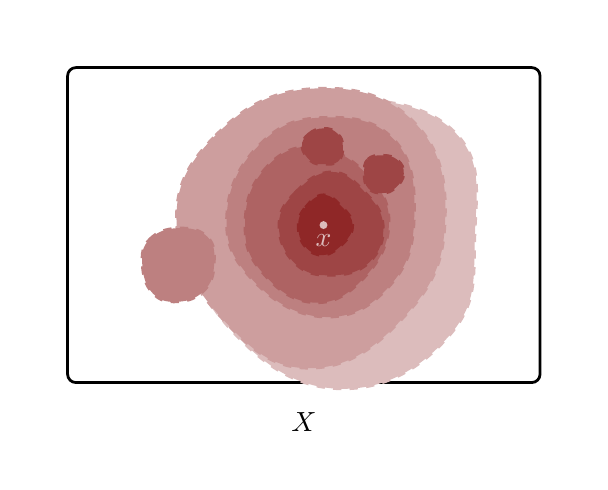
\begin{tikzpicture}[scale=1.0]
  
  \begin{scope}[shift={(0, 0)}]
    \draw[white] (-3.5, -3) rectangle (3.5, 2.5);
  
    \draw[rounded corners=3, color=black, line width=1] (-3, -2) rectangle (3, 2);
    \node at (0, -2.5) { $X$ };
  
    \foreach [count=\n] \r/\x/\y in {1.85/0.5/-0.15, 1.7/0.1/0, 1.25/0.25/0.15, 0.91/0.1/0, 0.63/0.35/0, 0.35/0.25/0} {
      \pgfmathsetmacro{\prop}{100 * (\n - 1) / 5}
      \colorlet{custom}{dark!\prop!light}; 
      \filldraw[custom, dashed, line width=1] 
        plot [smooth cycle, tension=0.75] coordinates { \randpoints{\x}{\y}{\r} } -- cycle;
    }
    
    \pgfmathsetmacro{\prop}{100 * (3 - 1) / 5}
    \colorlet{custom}{dark!\prop!light}; 
    \filldraw[custom, dashed, line width=1] 
      plot [smooth cycle, tension=0.75] coordinates { \randpoints{-1.6}{-0.5}{0.5} } -- cycle;

    \pgfmathsetmacro{\prop}{100 * (5 - 1) / 5}
    \colorlet{custom}{dark!\prop!light}; 
    \filldraw[custom, dashed, line width=1] 
      plot [smooth cycle, tension=0.75] coordinates { \randpoints{1}{0.65}{0.25} } -- cycle;
      
    \pgfmathsetmacro{\prop}{100 * (5 - 1) / 5}
    \colorlet{custom}{dark!\prop!light}; 
    \filldraw[custom, dashed, line width=1] 
      plot [smooth cycle, tension=0.75] coordinates { \randpoints{0.25}{1}{0.25} } -- cycle;
  
    \fill[light] (0.25, 0) circle (0.05) node[below] { $x$ };
  \end{scope} 
    
\end{tikzpicture}

\end{document}  